%!TEX root = ../template.tex
%%%%%%%%%%%%%%%%%%%%%%%%%%%%%%%%%%%%%%%%%%%%%%%%%%%%%%%%%%%%%%%%%%%%
%% chapter4.tex
%% NOVA thesis document file
%%
%% Chapter with lots of dummy text
%%%%%%%%%%%%%%%%%%%%%%%%%%%%%%%%%%%%%%%%%%%%%%%%%%%%%%%%%%%%%%%%%%%%

\typeout{NT FILE chapter4.tex}%

\chapter{Data Description and Management}
\label{cha:data}

The data used in this work focused mainly in the usage of biosignals. Some of the data used was searched with the intent of being related with data that can be acquired in occupational scenarios. This is to provide strong evidence that the methods developed, although applicable to any kind of time series, can be used for occupational health data as well. From public databases we used \gls{ecg}, \gls{abp}, \gls{emg}, \gls{acc} and \gls{gyro}. It is important to mention that for the sake of performance evaluation and comparison, several benchmark databases were used with a broad type of time series.

\section{Dataset 1 - UCR Benchmark}
\textbf{Description}\\
The University of California Riverside (UCR) Time Series Archive was introduced in 2002 and is one of the most used benchmarks for time series data mining tasks, specially for classification. The datasets are diverse in terms of data type, data domain, difficulty, number of classes and dimensionality\cite{ucr}. Several \textit{python} distributions make it available to download. In this thesis, all UCR archive datasets from the \textit{pyts} distribution were used for classification tasks. These represent 107 datasets from 18 different data types (audio, devices, \gls{ecg}, \gls{eog}, \gls{eeg}, \gls{har}, etc...), which also are from many different domains, such as medical, financial, motion, entomology, etc...\cite{ucr}. The list of datasets can be found on the following link \cite{ucr_site}.\\
\textbf{Purpose}\\
This dataset is the benchmark used in the context of time series classification to validate the proposed symbolic approach for this task. 
 
\subsection{Dataset 2 - Human Activity Recognition}

\textbf{Description}\\
The dataset was found on Kaggle and comprises data from 15 subjects that were performing 7 activities while wearing a sole wearable \gls{acc} mounted on the chest. The data was acquired at a constant rate of 52 Hz. The categories of activities are: \textit{(1) Working at computer, (2) Standing Up, Walking and Going Up/Down stairs, (3) Standing, (4) Walking, (5) Going Up/Down Stairs, (6) Walking and Talking with Someone, (7) Talking while Standing}. Each sample of the data gathered has a corresponding label from the performed activity \cite{dataset1}.\\
\textbf{Purpose}\\
This dataset was used in the context of novelty segmentation, to test the method in estimating transitions between the performed activities from the \gls{acc} data. 
 

%\section{UCI Machine Learning Repository}
%\label{subsec:uci}
%\textbf{Description}\\
%The University of California Irvine (UCI) Machine Learning is another well known benchmark for machine learning tasks. It does not focus solely on time series data mining, having datasets for time series, image, text or categorical data. This archive was created as an ftp in 1987 by a studen at UC Irvine, containing now 607 datasets. 
%\par
%From this archive, we focused in time series data for the validation of the proposed methods. More specifically, this repository contains time series that can be used to validate the proposed novelty and cyclic segmentation. We searched for multidimensional data that could be used for time series segmentation and had labeled data.
%\par
%The following datasets were used:

\section{Dataset 3 - Smartphone Dataset for Human Activity Recognition in Ambient Assisted Living}
\textbf{Description}\\
This dataset was gathered from an experiment on 30 volunteers. Each subject was wearing a smartphone on the waist while performing several activities: \textit{(1) Walking, (2) Walking Upstairs, (3) Walking Downstairs, (4) Sitting, (5) Standing and (6) Laying}. The activities were performed for approximately 60 seconds. The device recorded the internal \gls{acc} and \gls{gyro} data at a constant rate of 50 Hz. Each activity has been categorized and labeled on the acquired data \cite{dataset2, dataset2_2}.\\
\textbf{Purpose}\\
This dataset was used in the context of novelty segmentation \cite{dataset2, dataset2_2}.

\begin{figure}
\centering
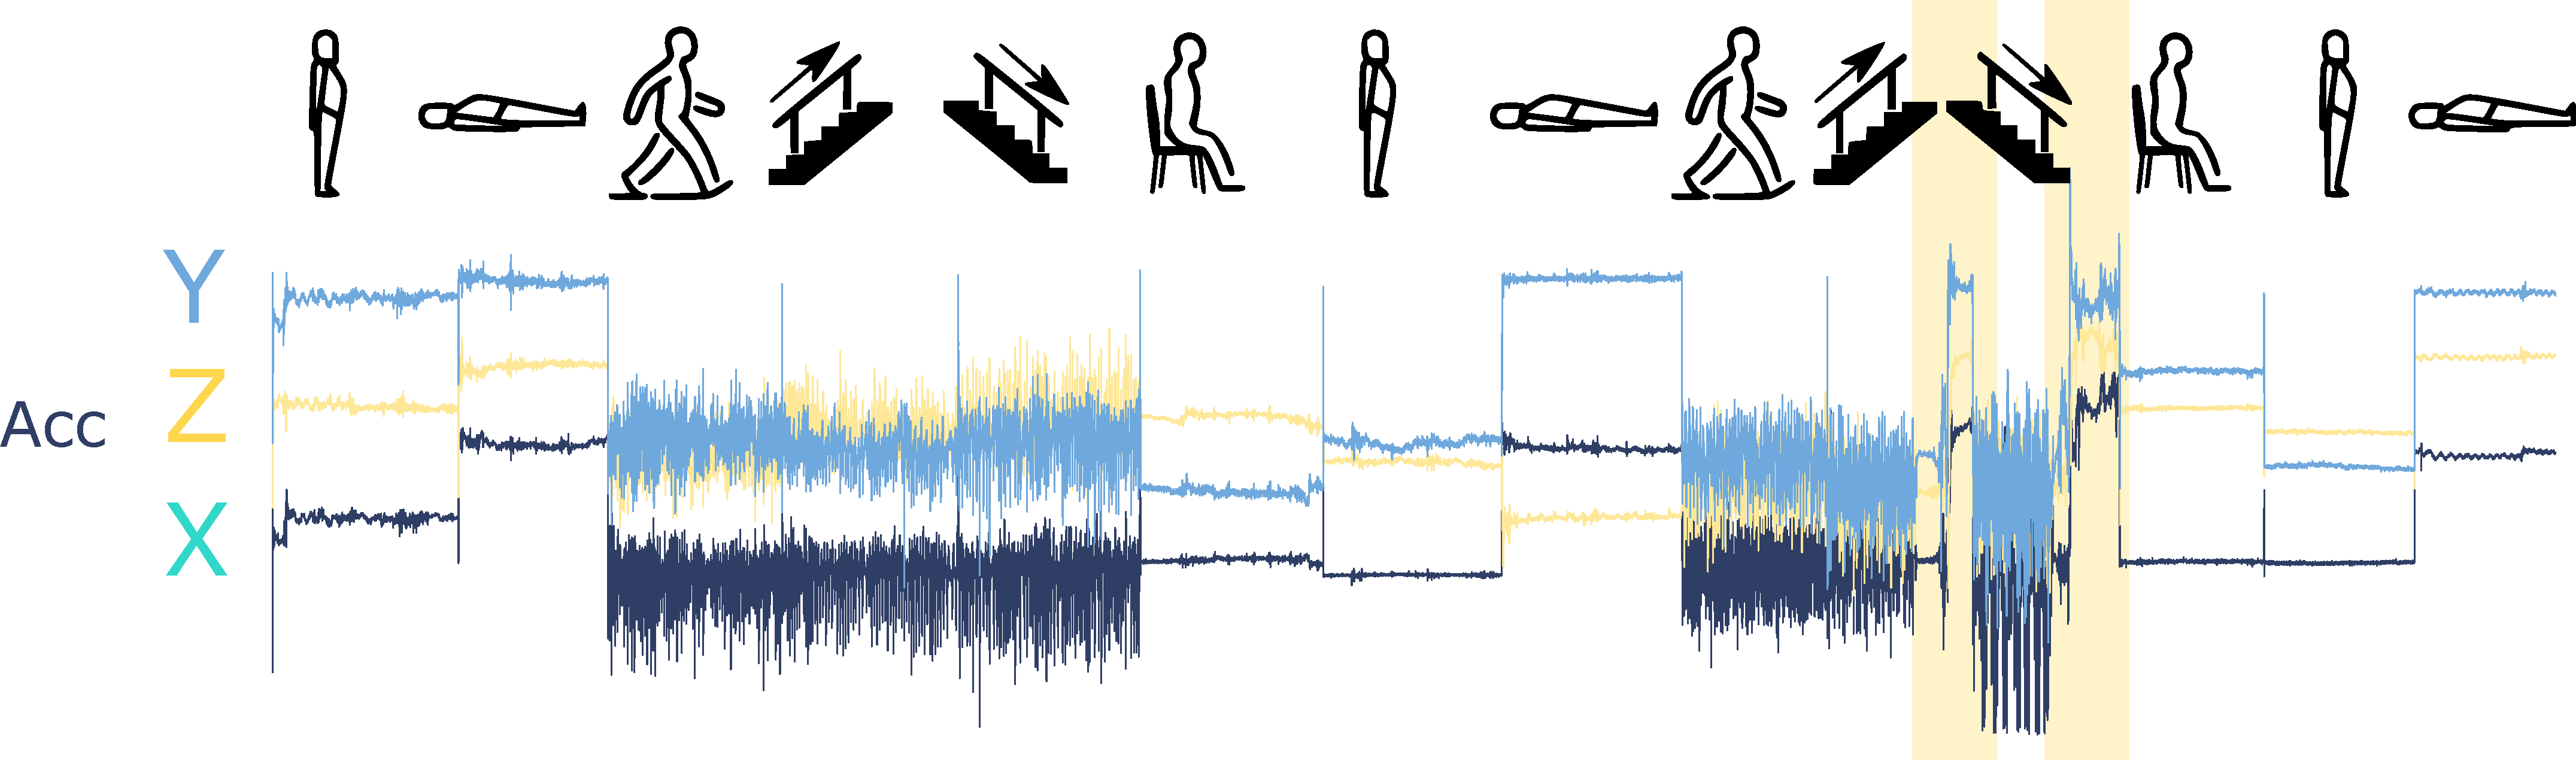
\includegraphics[width=\linewidth]{datasets/har_2_dataset.pdf}
\caption{Example of the signal for this dataset. It shows the 3 axis of the accelerometer signal and the corresponding labels in each section \cite{dataset2, dataset2_2}. Yellow areas indicate moments where there was a change on the signal not related with the labeled activity.}
\label{fig:har2_dataset}
\end{figure}
    
\section{Dataset 4 - Smartphone-Based Recognition of Human Activities and Postural Transitions}\\
\textbf{Description}\\
The dataset was built in the context of human activity recognition experiments. These were carried out with a group of 30 volunteers that performed a protocol with six basic activities: three static postures (standing, sitting, lying) and three dynamic activities (walking, walking downstairs and walking upstairs). Additionally, the experiment also included postural transitions that occurred between the static postures. These are: stand-to-sit, sit-to-stand, sit-to-lie, lie-to-sit, stand-to-lie, and lie-to-stand. The data was collected with a smartphone (Samsung Galaxy S II) mounted on the waist of each subject. The data from a 3-axis accelerometer and 3-axis gyroscope was gathered at a constant rate of 50Hz. The experiments were video-recorded to label the data manually \cite{dataset3}.\\
\textbf{Purpose}\\
This dataset was used in the context of novelty segmentation \cite{dataset3}.

\begin{figure}
\centering
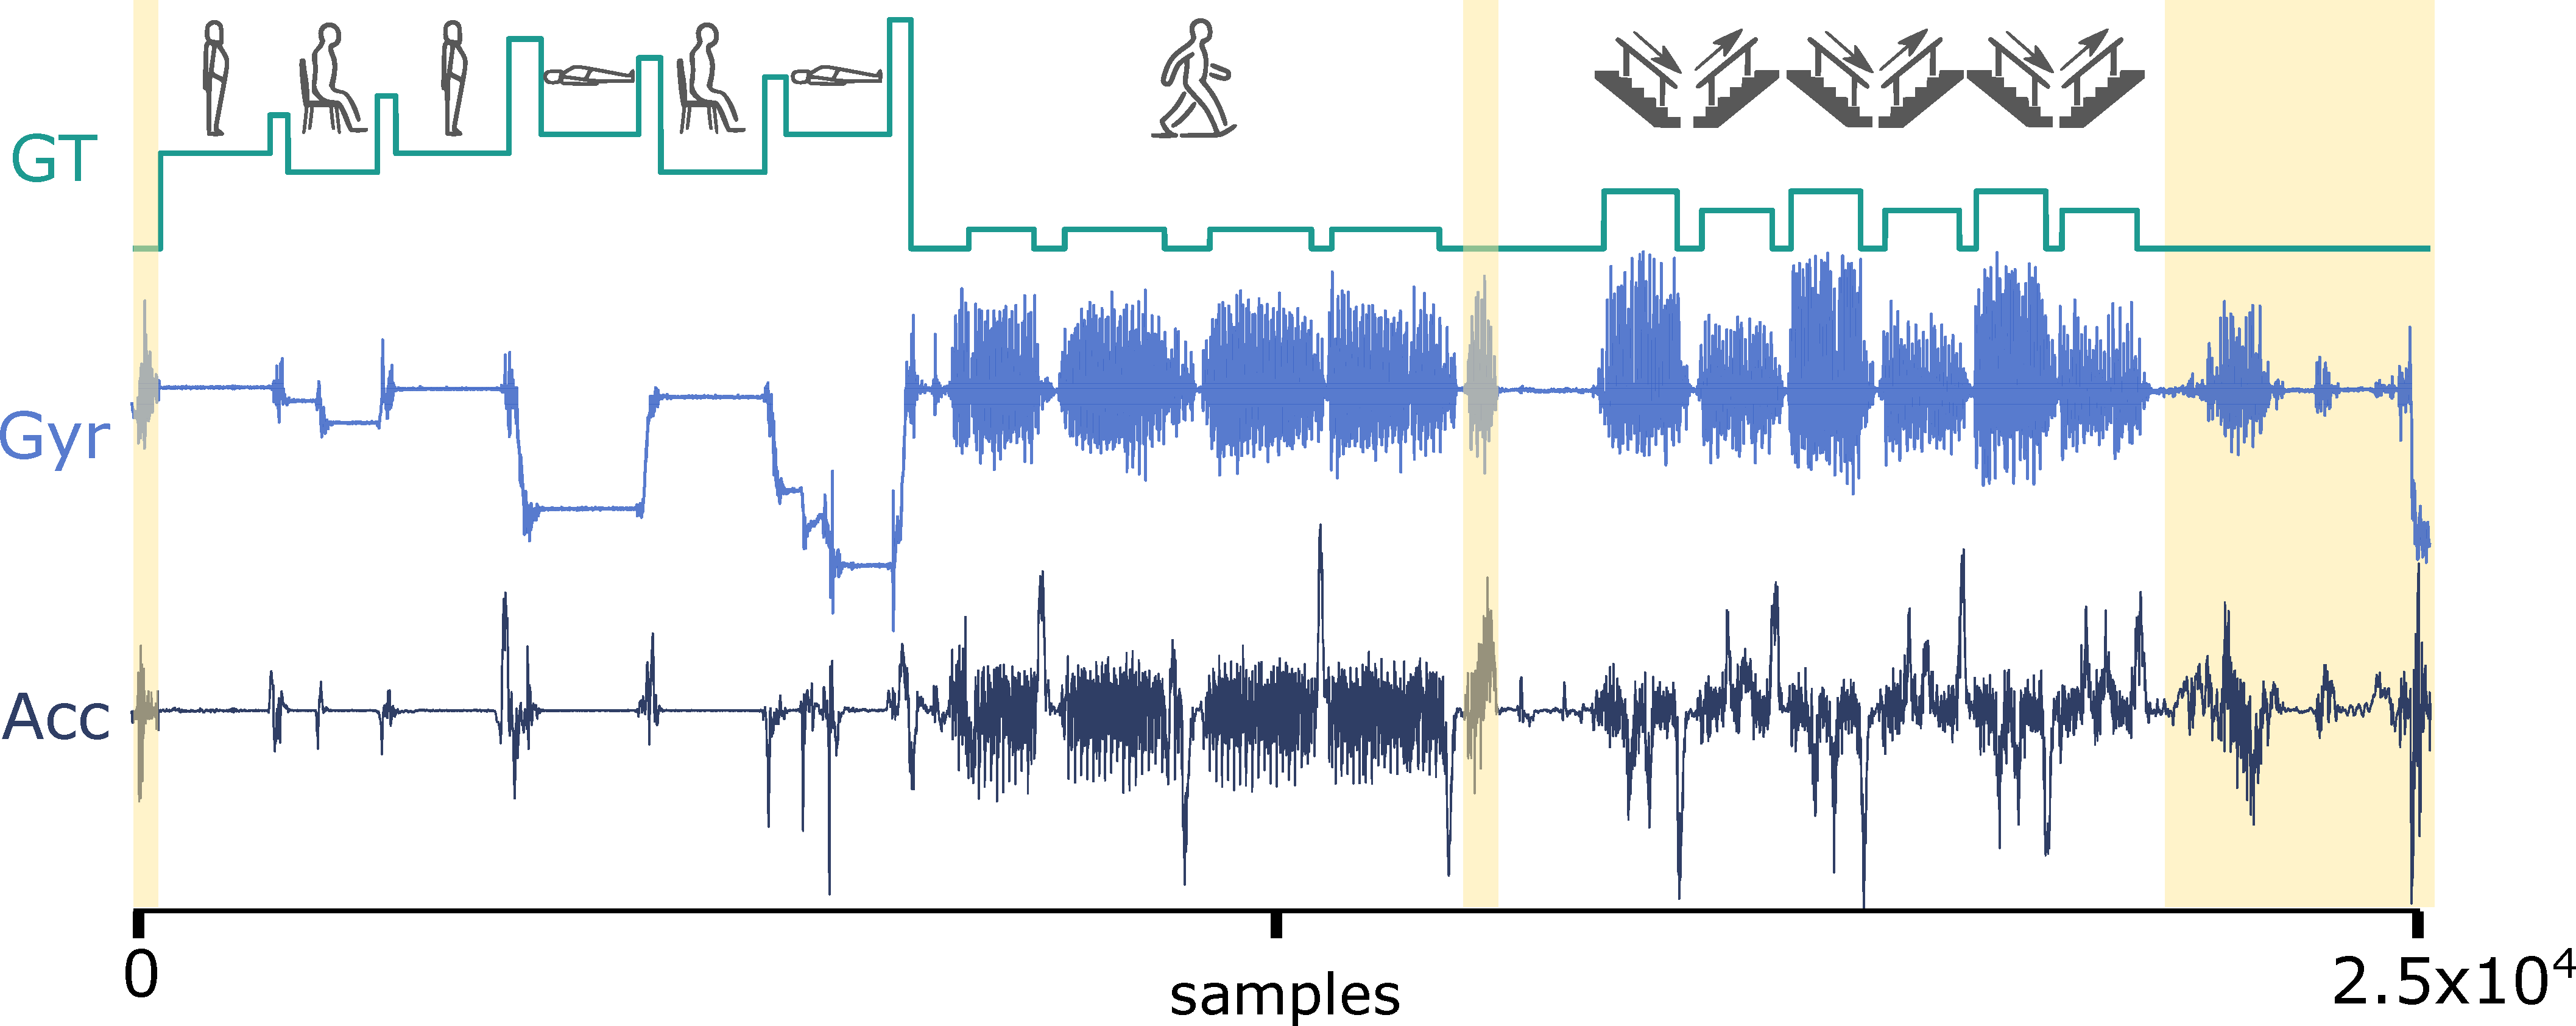
\includegraphics[width=\linewidth]{datasets/har_1_dataset.pdf}
\caption{Example of the signal for this dataset. It shows one axis for the \gls{acc} and \gls{gyro} signals and the corresponding labels in each section \cite{dataset3}. In this datasets, labels also highlight posture transitions, such as \textit{Standing to Sitting}. Yellow areas indicate moments where there is activity but the signal was not labeled.}
\label{fig:har1_dataset}
\end{figure}    
    
\section{Dataset 5 - Wireless Sensor Data Mining (WISDM) Smarphone and Smartwatch Activity Biometrics Dataset}\\
\textbf{Description}\\
The raw data from the accelerometer and gyroscope sensors is collected from a smartphone and smartwatch at a rate of 20Hz. This experiment was conducted on 51 participants as they performed 18 activities, each for a duration of 3 minutes. Each sample of the data was labelled based on the activity it corresponds to. The activities are diverse and include dribbling, eating, jogging, sitting, walking on stairs, standing, walking, among others \cite{dataset4}.\\
\textbf{Purpose}\\
This dataset was used in the context of novelty segmentation in complex real-life scenarios.

\begin{figure}
\centering
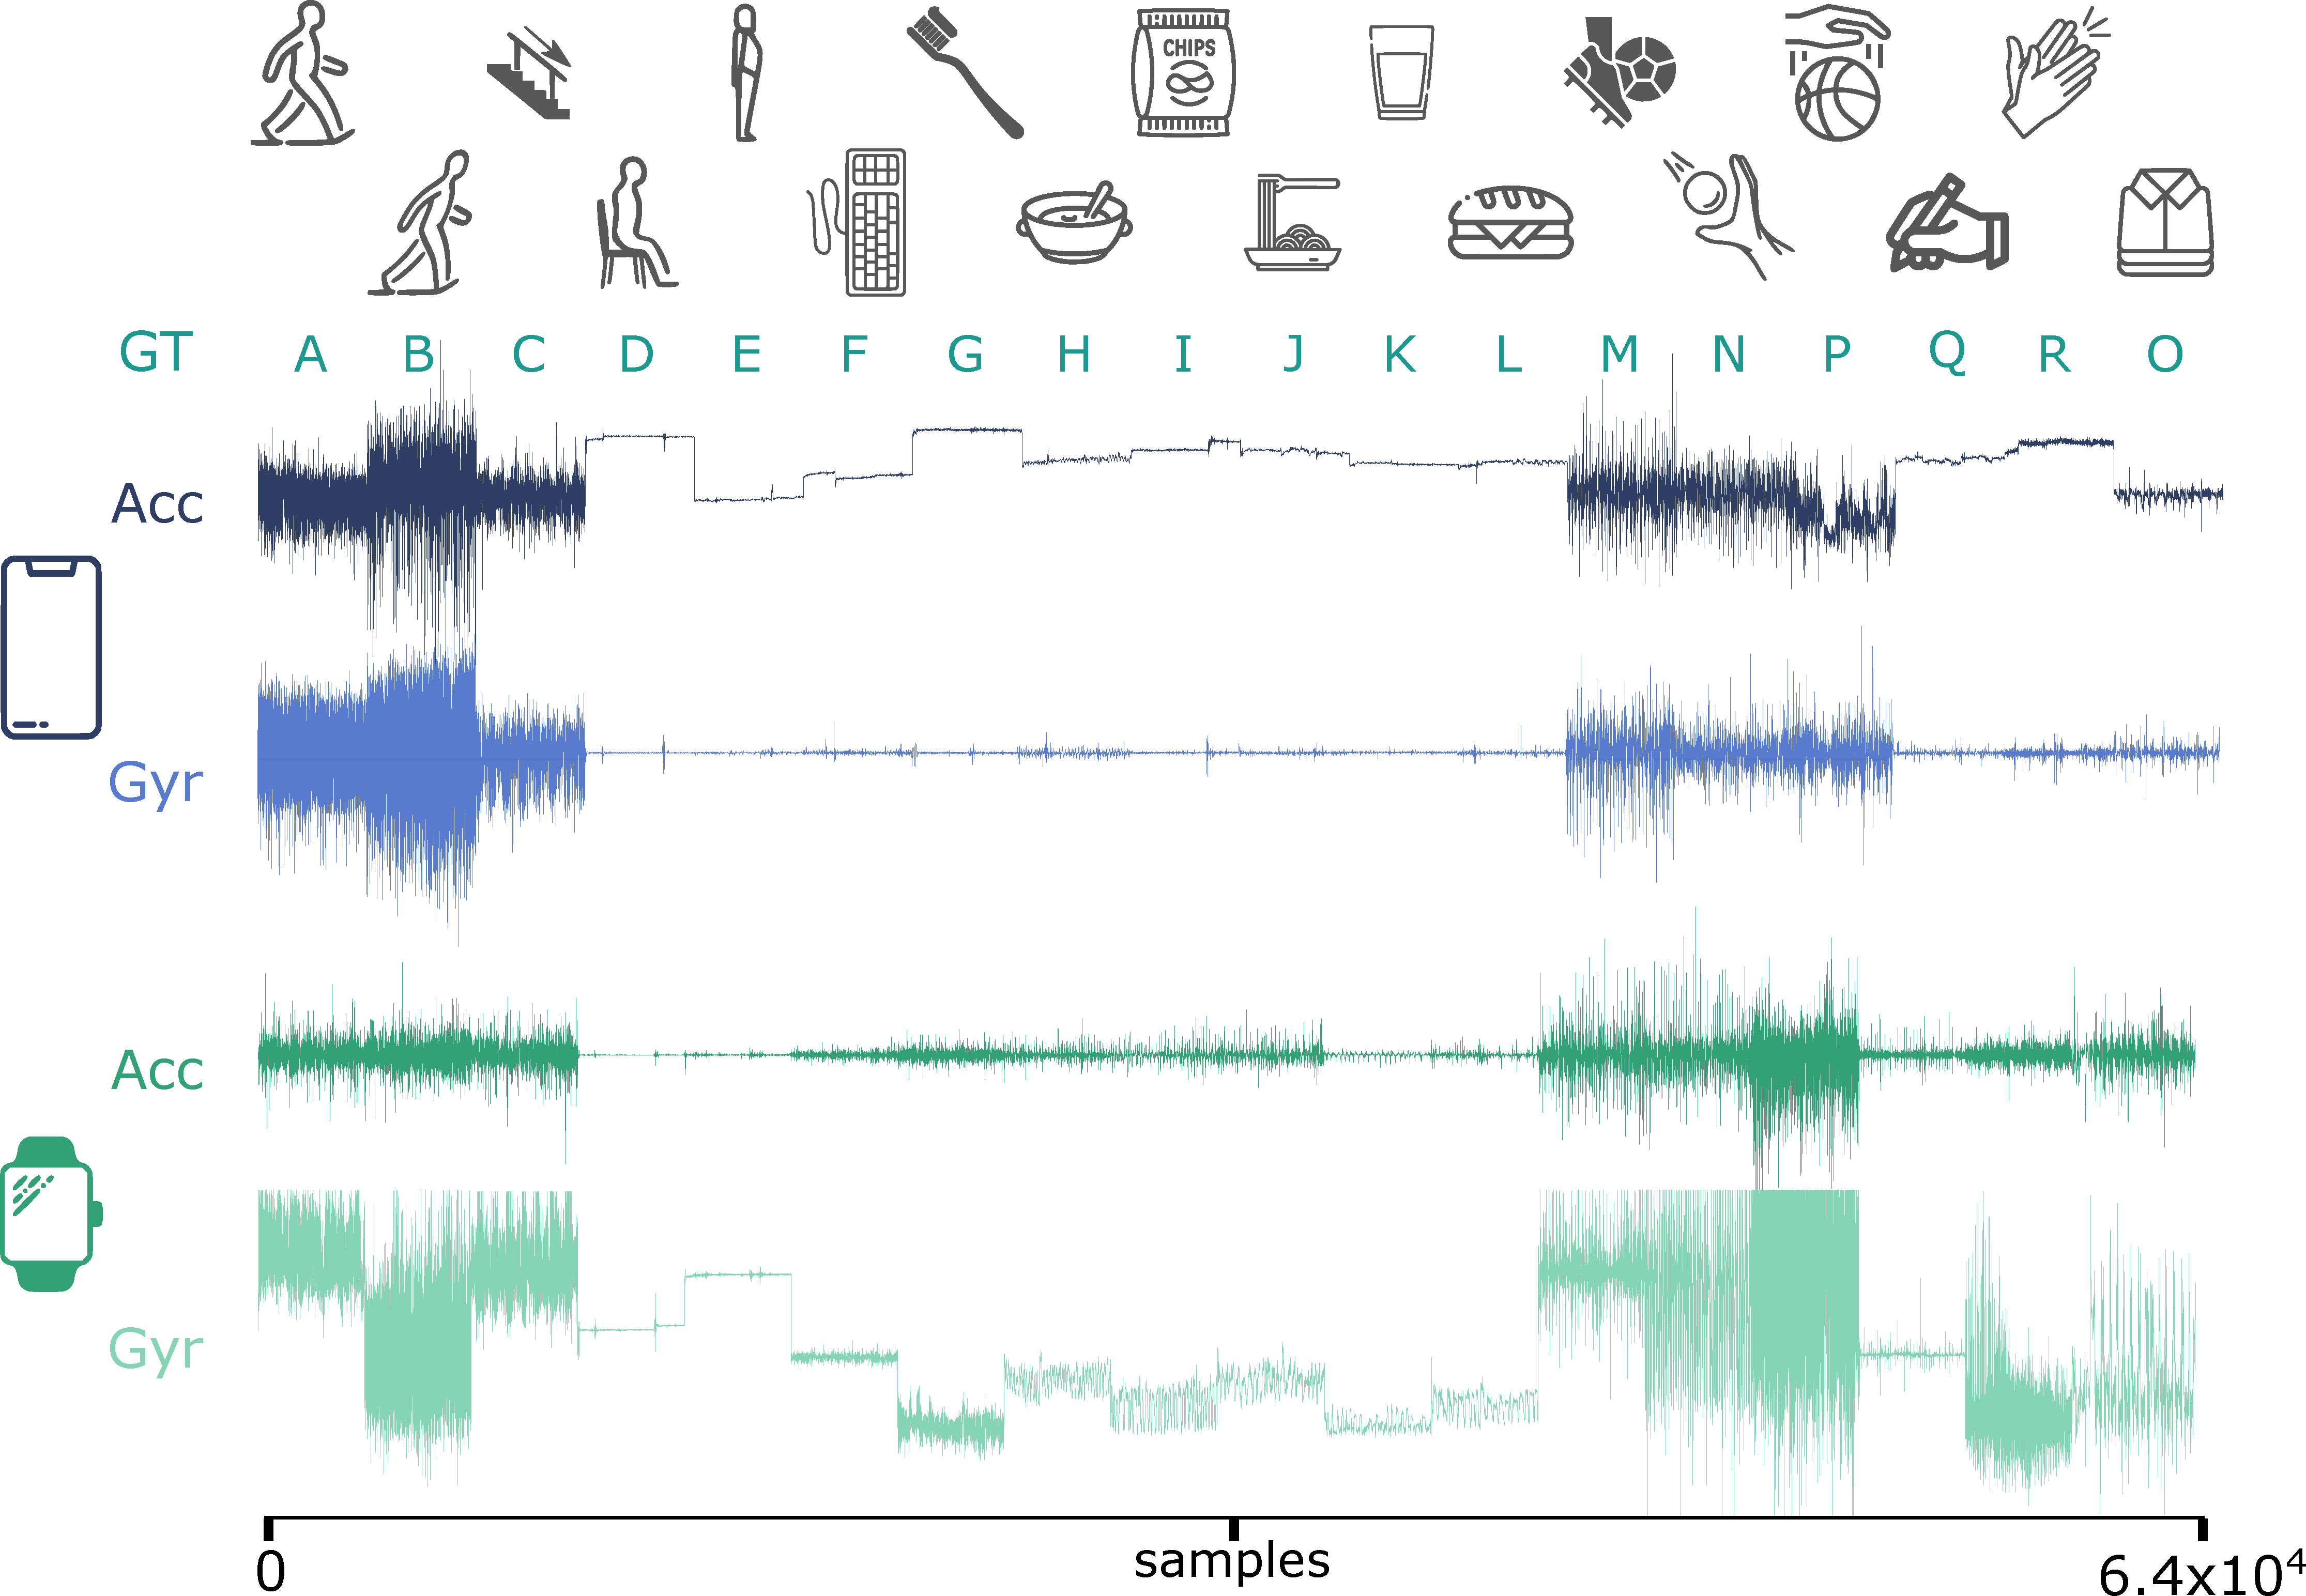
\includegraphics[width=\linewidth]{datasets/wisdim_dataset.pdf}
\caption{Example of the signal for this dataset. It shows one axis of each type of data acquired, for both smartphone and smartwatch. The activities are highlighted as well and labeled as: A - walking, B - running, C - walking on stairs, D - sitting, E - standing, F -   typing, G - brushing, H - eating soup, I - eating chips, J - eating pasta, K - drinking, L - eating a sandwich, M - kicking, N - catching a ball, P - dribbling, Q - writing, R - clapping, O - iron \cite{dataset4}.}
\label{fig:wisdim_data}
\end{figure}

\section{Dataset 6 - EMG Data for Gestures}\\
\textbf{Description}\\
This dataset has EMG signals for recording patterns, by using a MYO Thalmic bracelet worn on a user's forearm. The bracelet is equipped with eight sensors equally spaced around the forearm that simultaneously acquire electromyographic signals. The dataset has raw EMG data from 36 subjects while they performed series of static hand gestures. The subject performs two series, each of which consists of six basic gestures. Each gesture was performed for 3 seconds with a pause of 3 seconds between gestures. The data was collected with a fixed sampling frequency of 200 Hz \cite{dataset5}.\\
\textbf{Purpose}\\
This dataset was used in the context of novelty segmentation, to test the method in estimating transitions between the activation (onset) and relaxation (offset) of the muscular activity.

\begin{figure}
\centering
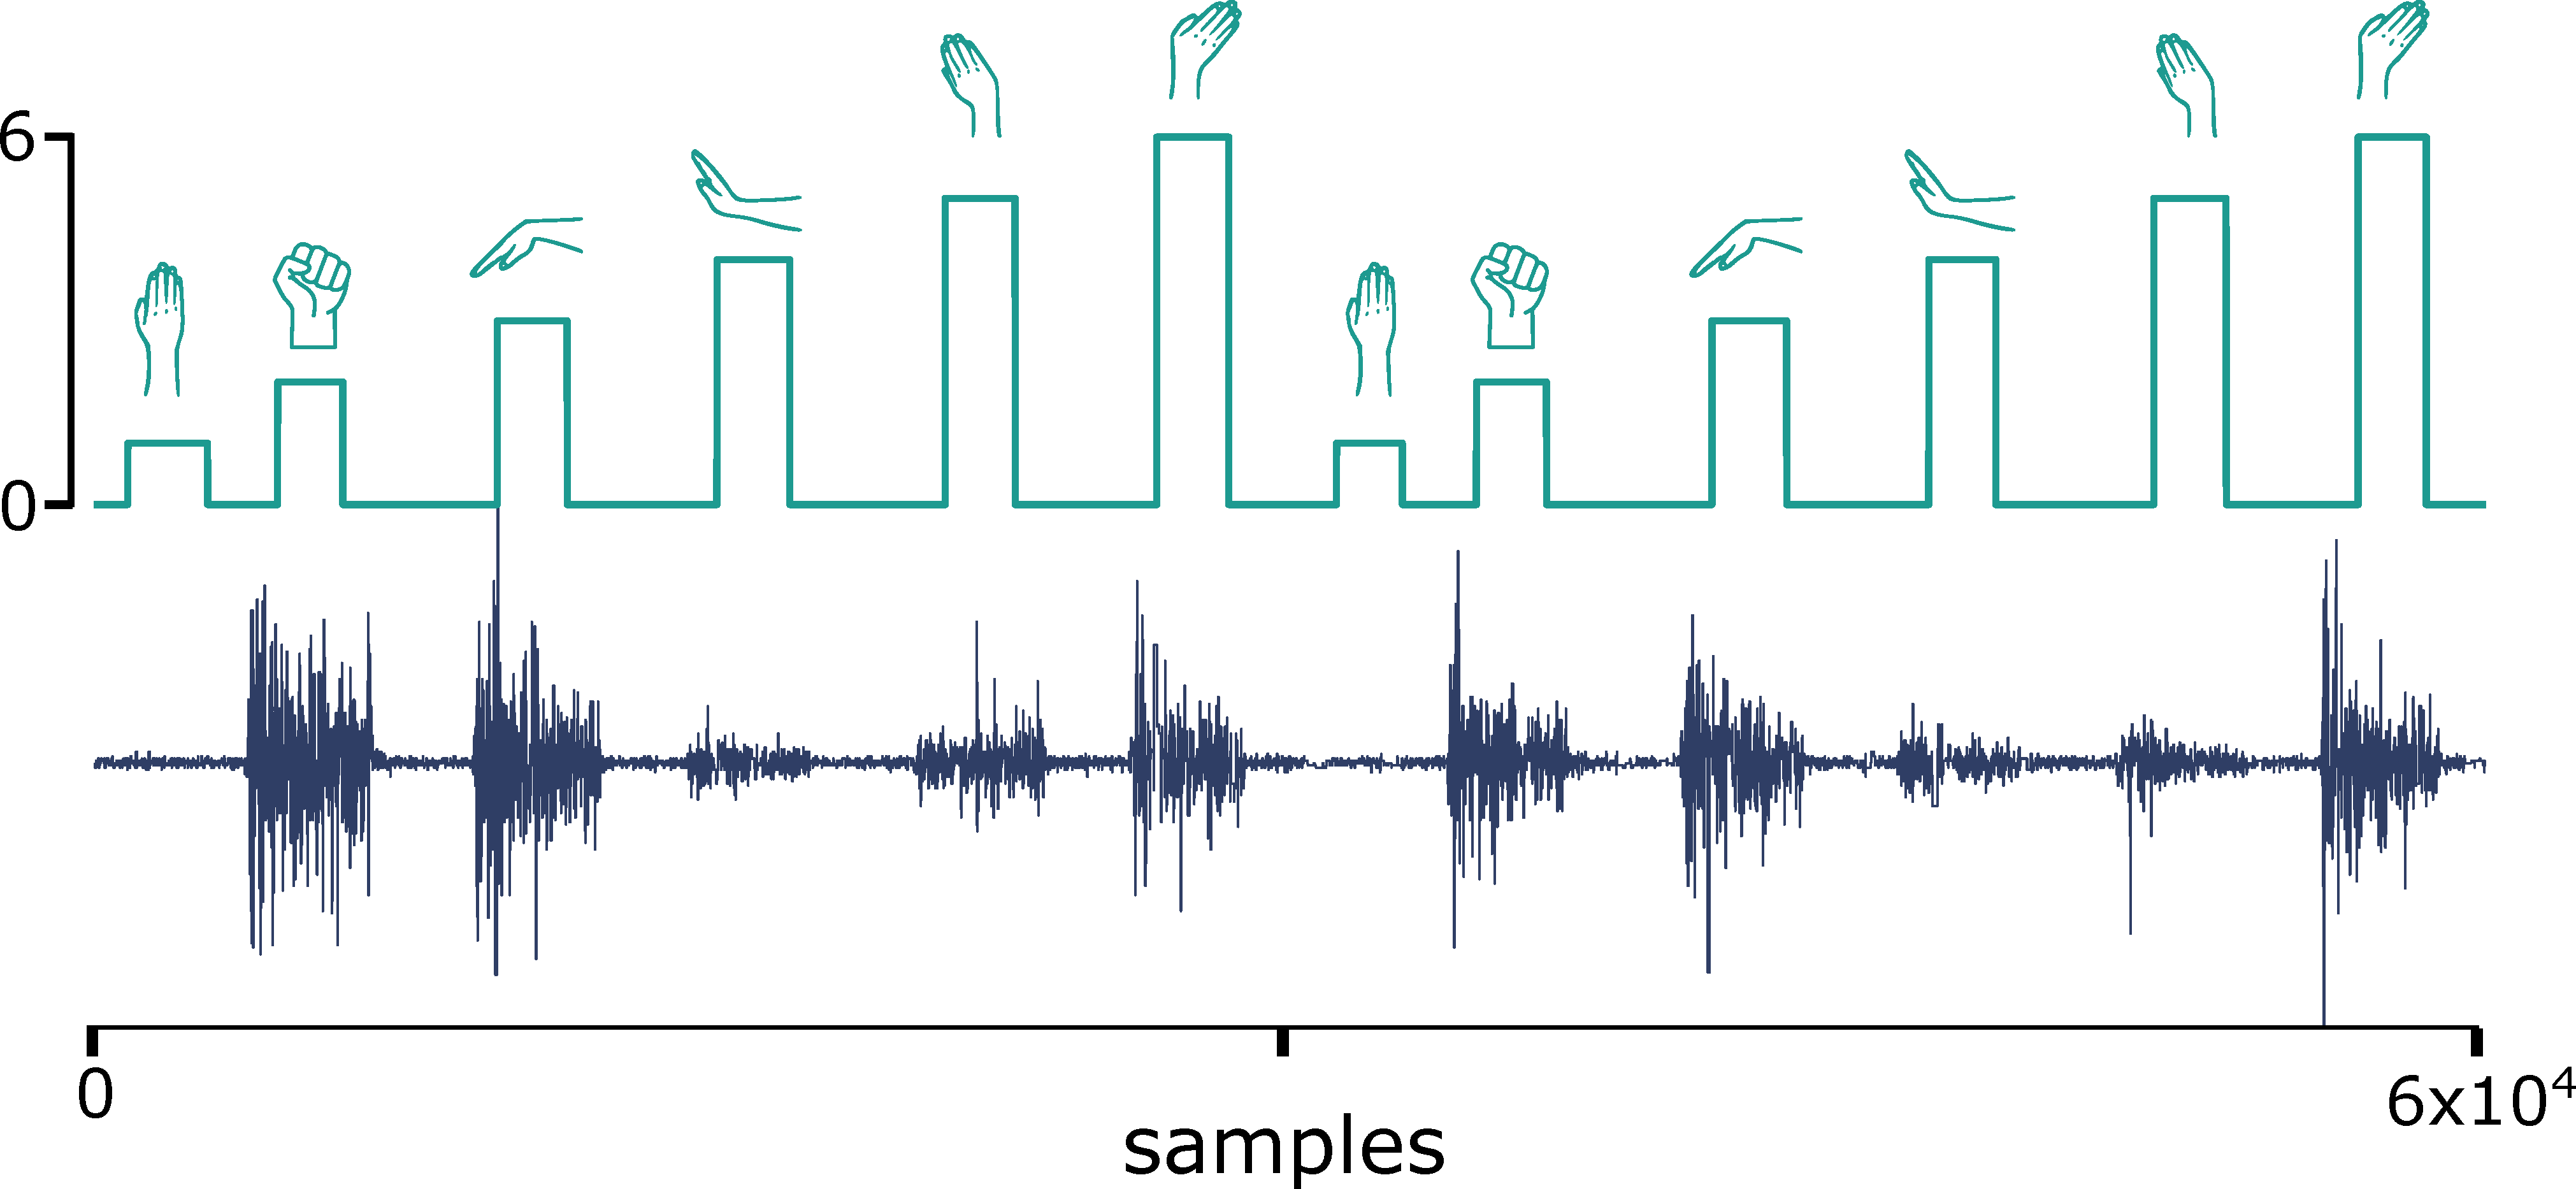
\includegraphics[width=\linewidth]{datasets/emg_dataset.pdf}
\caption{Example of the \gls{emg} data and the corresponding hand postures.}
\label{fig:emg_dataset}
\end{figure}

As indicated in Figure \ref{fig:emg_dataset}, the ground truth would have considered as events the absence of activity (which the original dataset uses because it was designed for a classification problem). In this case, we did not considered these events in our ground truth for this dataset for the problem of segmentation.    

%\section{Physionet}
%\label{subsec:physionet}
%
%Physionet is a platform where public datasets from the medical domain (mostly physiological signals) are available. In this thesis, we used several datasets to test the developed methods.

\section{Dataset 7 - MIT-BIH Noise Stress Test Database}\\
\textbf{Description}\\
The dataset comprehends 12 half-hour \gls{ecg} recordings and 3 half-hour recordings of noise typical in ambulatory \gls{ecg} recordings. The noise recordings were made using physically active volunteers and standard \gls{ecg} recorders, leads, and electrodes. The three noise records were assembled from the recordings by selecting intervals that contained predominantly baseline wander (in record 'bw'), muscle (EMG) artifact (in record 'ma'), and electrode motion artifact (in record 'em'). Two clean \gls{ecg} signals were selected and noise was added with different signal-to-noise ratios (SNR) \cite{dataset6, PhysioNet}.\\

\begin{figure}
\centering
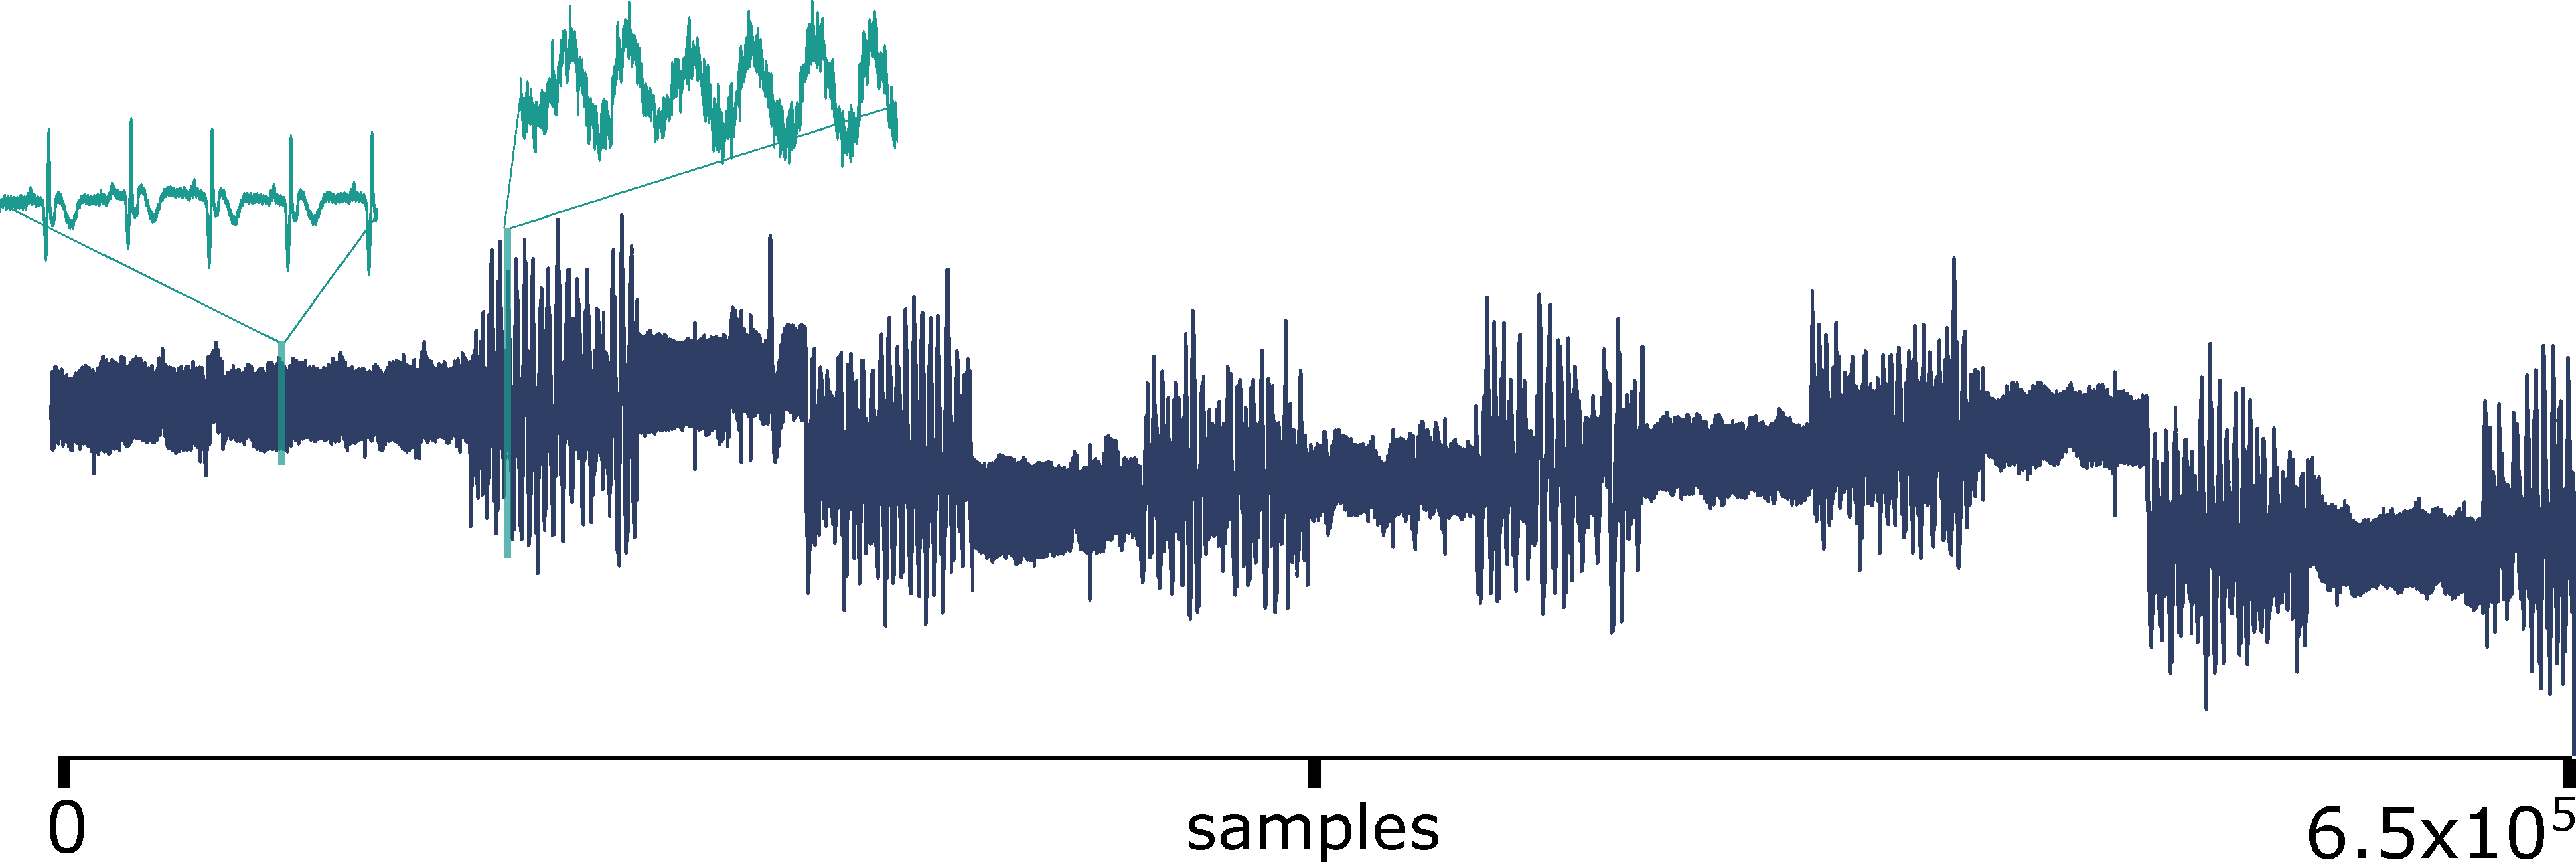
\includegraphics[width=\linewidth]{datasets/ecg_noise1.pdf}
\caption{Example of an \gls{ecg} record contaminated with noise. Two sections are highlighted showing the clean and contaminated area of the signal. \cite{dataset7}}
\label{fig:ecg1_dataset}
\end{figure}

\textbf{Purpose}\\
This dataset was used in the context of novelty segmentation, to test the method in estimating transitions to and from noise sections of the signal.
    
\section{Dataset 8 - Motion Artifacted Contaminated \gls{ecg}}\\
\textbf{Description}\\
This dataset has short duration \gls{ecg} signals, which were recorded from a healthy 25-year-old male performing different physical activities (standing, walking and single jump) to study the effect of motion artifacts on \gls{ecg} signals and their sparsity. The dataset was acquired with a sampling rate of 500 Hz and 16 bit resolution. For this exercise, only the records with jump were used \cite{dataset7, PhysioNet}.\\

\begin{figure}
\centering
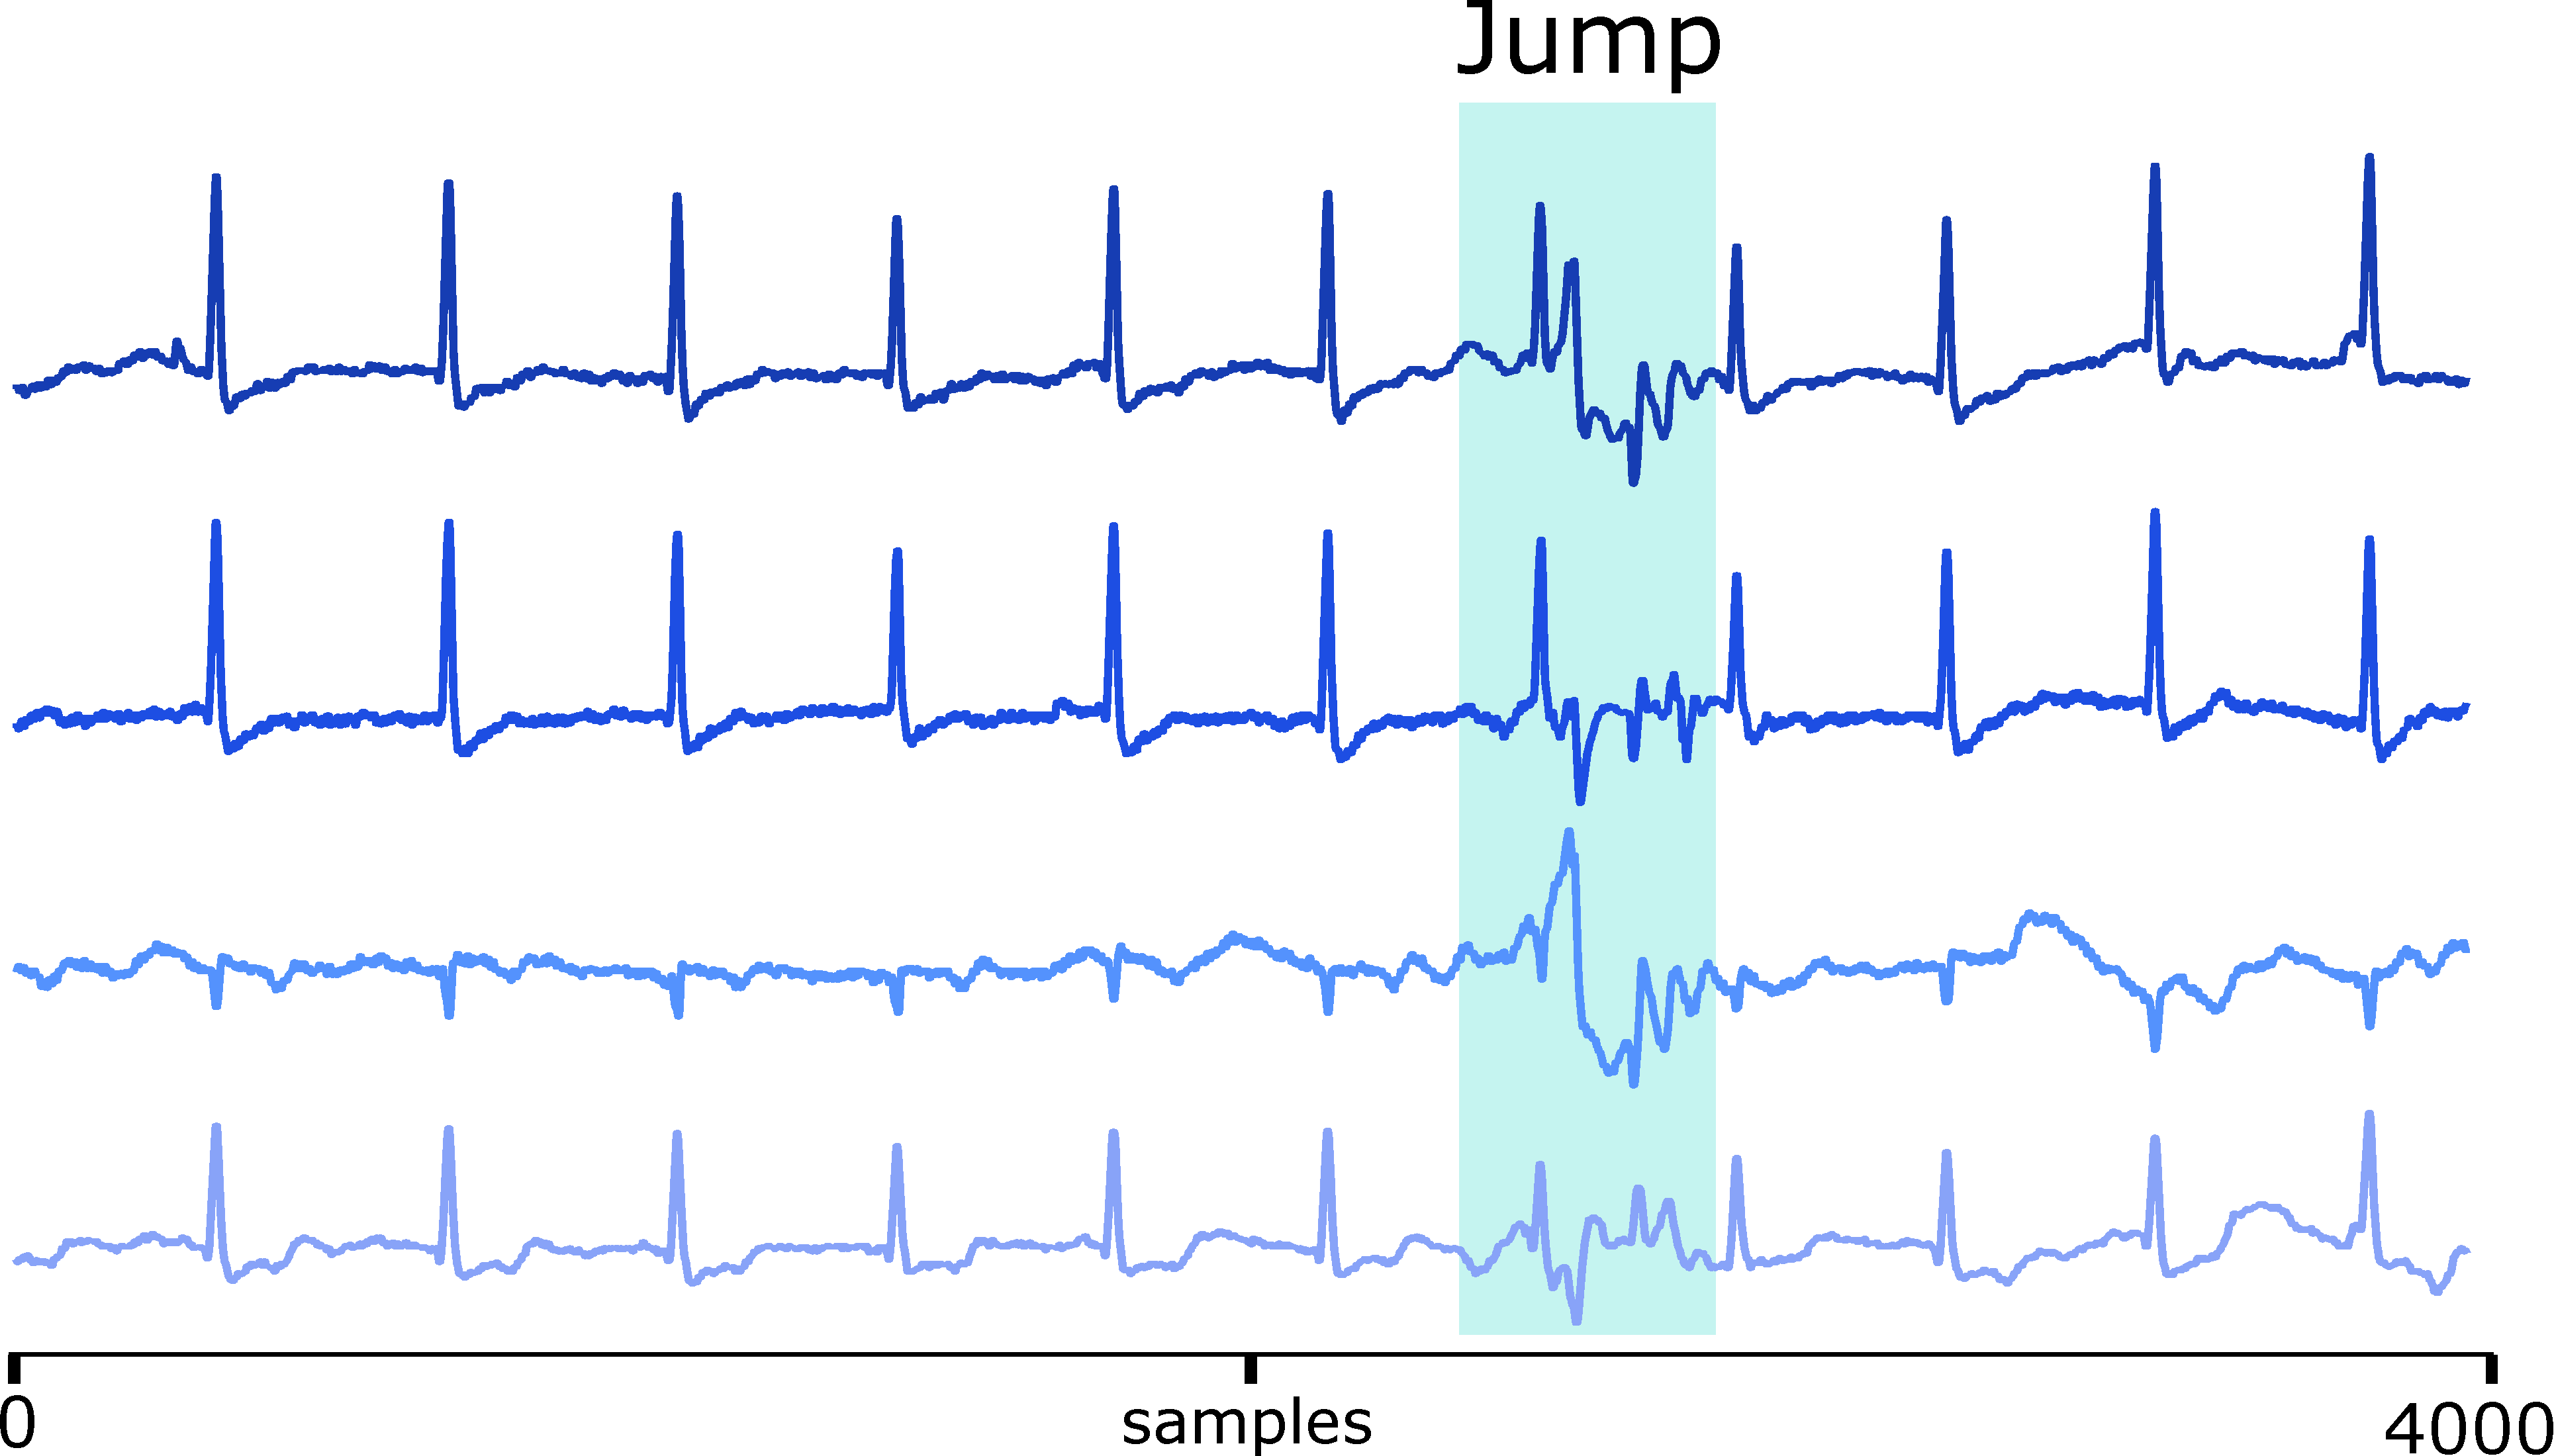
\includegraphics[width=0.85\linewidth]{datasets/ecg_noise2.pdf}
\caption{Example of an \gls{ecg} signal contaminated with motion artifacts. The artifact is visible due to a jump from the subject.}
\label{fig:ecg2_dataset}
\end{figure}

\textbf{Purpose}\\
This dataset was used in the context of change point detection, to test the method in estimating transitions to and from noise sections of the signal.

\section{Dataset 9 - St Petersburg INCART 12-lead Arrhythmia Database}\\
\textbf{Description}\\
This dataset has \gls{ecg} signals from patients undergoing tests for coronary artery disease. 75 annotated recordings were extracted. Each record is 30 minutes long and has 12 leads, each sampled at 257 Hz. The annotations include beats as well as relevant artifacts/occurrences present on the signal, such as arrhythmia \cite{PhysioNet}. Records \textit{I02, I04 and I09} were used.\\
\textbf{Purpose}\\
This dataset was used in the context of pattern search with \gls{quots} for the detection of different types of arrythmia.


\section{Dataset 10 - Alan Turing CPD Benchmark}
\label{sec:dataset8}
\textbf{Description}\\
The Alan Turing Change Point Detection Benchmark is a recent dataset used to have a standard reference for change point segmentation tasks. The benchmark was created in 2020 and provides 42 datasets, being 42 univariate time series and 4 multi dimensional time series. The dataset comprises several time series from real-world data. It was built from a project of the Alan Turing Institute to have a repository for the evaluation of change point detection algorithms. The available benchmark page was used to get access to the datasets, and run the performance metrics developed. This way, the performance of the proposed method is compare with the performance of several existing methods \cite{cpd_alan}.\\
\textbf{Purpose}\\
This dataset has ground-truth events for each time series. The performance of several existing methods is available and used to compare with the performance of the proposed method on the same time series.

\section{Dataset 11 - HCILab Behavioural Driving Dataset}
\textbf{Description}\\
It is a public dataset that studied ways of assessing the driver's workload combining auto telemetry data with physiological sensors. The authors conducted a real world driving experiment with 10 participants measuring a variety of physiological data as well as a post-hoc video rating session \cite{hcilab}. It includes a variety of physiological signals, such as \gls{ecg} and corresponding heart rate, \gls{scr} and body temperature. In addition, it collected driving speed and GPS location. The map of the driving site can be seen at \cite{hcilab}\\
\textbf{Purpose}\\
This dataset was used for \gls{quots} in pattern search. For the example presented we used the data of participant number 10 \cite{hcilab}.

\subsection{Dataset 12 - CSL-Share Dataset}
\textbf{Description}\\
For this thesis, there were allowed access to inertial acquisitions made in the context of human activity recognition. The database used was obtained on the scope of the \textit{Arthrokinemat} project whose main objective was the development of a learning adaptive sensor-based measurement system to prevent osteoarthritis\cite{arthrokinemat}. More specifically, the recording was made for the work of \cite{Liu2019}, which introduces a human activity recognition system able to recognize between a list of several daily activities.
\par
A set of multiple Biosensors were used, with various internal characteristics. Beginning with two \textit{8 channel PLUX hubs} a device which allows for the wireless acquisition of biosensors via Bluetooth, with them being part of the \textit{biosignals plux Research Kits}. From both \textit{plux hubs} there were used two 3-axial \gls{acc} sensors, 4 sets of \gls{emg} sensors and an electrogoniometer. Adding to these sensors there were also used 4 other types of biosensors: one airborne microphone, one piezoelectric microphone, two 3-axial gyroscopes and one force sensor. This setup was used to perform 18 different activities, namely \textit{Sit}, \textit{Sit-to-Stand}, \textit{Stand}, \textit{Stand-to-Sit}, \textit{Stair-Up}, \textit{Stair-Down}, \textit{Walk}, \textit{Curve-Left-Step}, \textit{Curve-Left-Spin}, \textit{Curve-Right-Step}, \textit{Curve-Right-Spin}, \textit{Run}, \textit{V-Cut-Left}, \textit{V-Cut-Right}, \textit{Lateral-Shuffle-Left}, \textit{Lateral-Shuffle-Right}, \textit{Jump-One-Leg}, \textit{Jump-Two-Leg}. As a disclaimer, \textbf{lateral-shuffle-left/right} is a motion usually done in sports that describes the subject's lateral movement of the left/right foot, with the other foot following along and continuing the shuffling in the same direction. \textbf{V-cut-left/right} means that the subject changes his direction by 90\degree at jogging speed \cite{dataset_hui}.\\
\textbf{Purpose}\\
This database was used to study how the algorithm could be used to detect periodic events with different levels of motion cycle complexity.


\section{Dataset 13 - Industrial Job Dataset}
\label{sec:industry}
\textbf{Description}\\
During the period of this thesis, a private dataset was acquired at Volkswagen Autoeuropa in the context of this thesis and a master thesis from \cite{santos2019}. The purpose was to test a wearable system capable of calculating the ergonomic risk through direct measures from inertial sensors. The technological setting was provided by a sensing framework named Internet of Things in Package (IoTiP), designed and provided by Fraunhofer AICOS. IoTiP is a system that intends to combine hardware, firmware and software components to promote the field "Internet of Things"\cite{FraunhoferAICOS}. For this work, the technology setting consisted on 4 9-\gls{dof} \gls{imu} sensors (composed internally by a triaxial \gls{acc}, triaxial \gls{gyro} and triaxial \gls{mag}) and an Android wireless communication system. The last one was made through an application called Recorder, also developed by Fraunhofer AICOS.\cite{santos2019}.
\par
The acquisition was made in a \textit{Volkswagen Industrial} assembly line where 12 manufacturing workers performed their work tasks while having attached 4 \gls{imu} sensors in their upper body segments. During the acquisition, the subjects performed various tasks in multiple workstations. Relevantly to this thesis, the database comprehends three different workstations from \textit{Bodyshop assembly line}, a section where cars' doors were assembled: 1) Liftgate workstation, where back doors are mounted; 2) Fender workstation, involving front door tasks and 3) Doors workstation, which demanded tasks on the front doors and in the cars' hood \cite{santos2019}. The acquisitions made involved a total of 6 operators with each one performing at least 2 different workstations. The various acquisitions were simultaneously filmed, and to synchronize the ground manual annotations of the data, at the beginning and end of the acquisition the subjects were asked to stay, firstly, in a neutral anatomic position and then perform a T pose (calibration position). There were also registered some details regarding their anthropometric characteristics.
\par
The mentioned study was centered on the ergonomic assessment of the dominant arm. For this reason, the \gls{imu}s  were attached in: 1) the posterior side of the hand, 2) posterior side of the forearm and 3) posterior side of the arm and a final one 4) placed in the anterior side of the thorax area. All of the devices were attached with elastic bands, in such a way that all had their Y-axis pointed up while in a neutral anatomical position. Additionally, a Smartphone was attached to the trunk of the workers as well, working as an additional \gls{imu}, from which the position of the arm in regards to the body posture was calculated. Each one of these 4 \gls{imu} devices had incorporated within them 3 triaxial sensors (\gls{acc}, \gls{gyro}, \gls{mag}).\\
\textbf{Purpose}\\
This database was used to study the application of the algorithm to detect (1) Working Periods with the novelty function, (2) Periodic Working Cycles with the similarity function and (3) Search by example. The data was annotated based on video inspection.
\par
Some important notes regarding exceptions found in sensors:
\begin{enumerate}
\item Despite the actual acquisition having three sensors \gls{acc}, \gls{gyro} and \gls{mag}, only the \gls{acc} and \gls{gyro} sensors were considered for this study as this had the best behaviour, and the \gls{mag} was acting in an erratic manner.
\item The two workstations of operator 2 were made during the same acquisition, resulting in a single time series, where the subject performed two different types of active work motions.
\item In operator 2 workstations 1\& 2 the torso was not considered, due to malfunction.
\end{enumerate}
More details regarding the dataset and the acquisition process can be found at \cite{sara2019, santos}.


\subsection{Notes for Ground Truth Annotations on Novelty Segmentation}

Regarding the proposed method for novelty segmentation, the datasets used were mostly designed for classification tasks. Therefore, these were labeled with categorical values for each sample of the time series. As the problem of novelty segmentation requires the detection of specific samples of the signal, we adapted the labels of the datasets to fit the purpose of segmentation. This was made by only keeping the transitions between categories of labels, for example, in Figure \ref{fig:har1_dataset}, the ground-truth (GT) is categorical. For evaluation purposes, the ground-truth was converted to a binary signal, where categorical transitions were valued to \textbf{1}, to keep only the position of the change, and not the category. This is valid for segmentation purposes only.